\chapter{Introduction}\label{ch:introduction}

\vspace*{-50pt}

\begin{figure}[ht]
        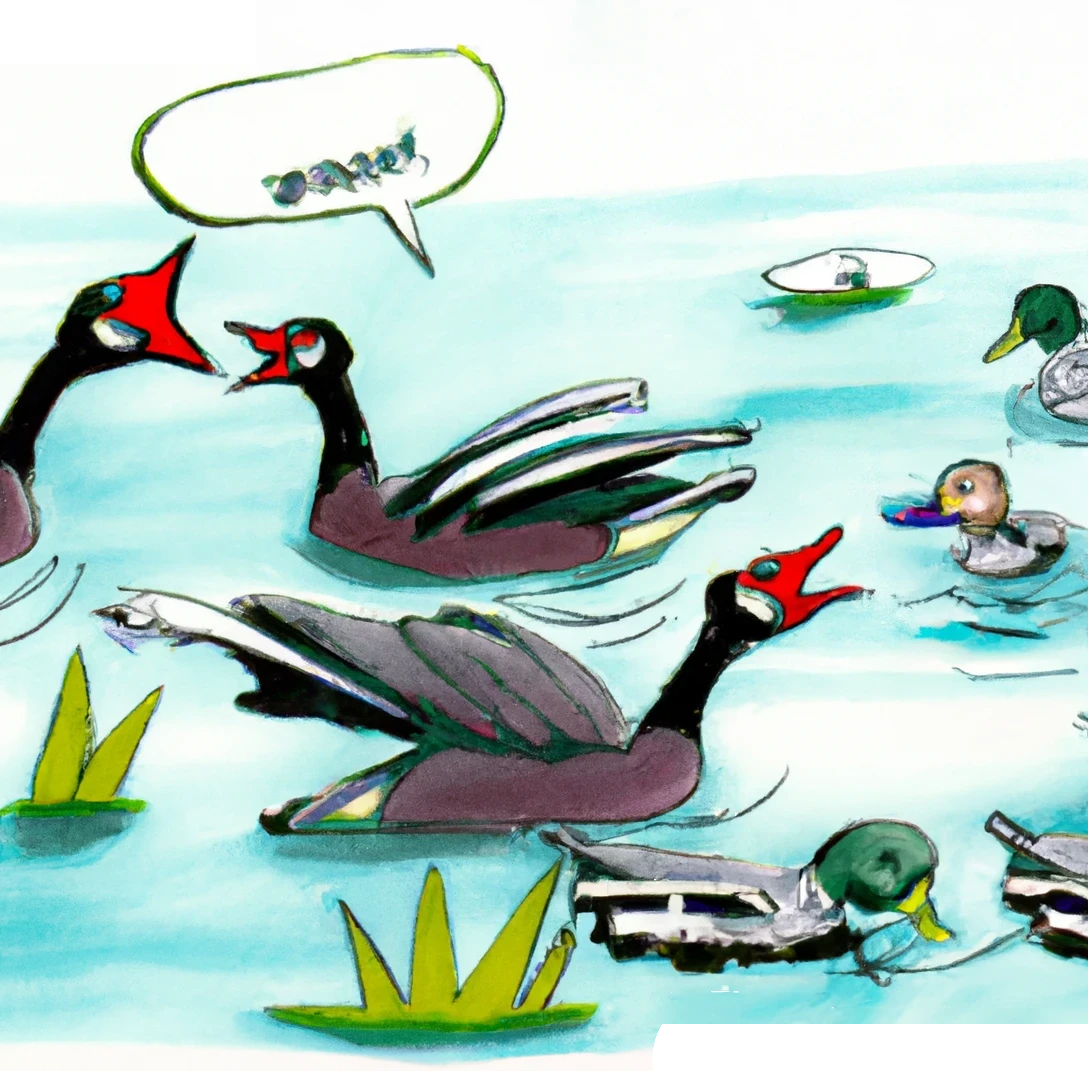
\includegraphics[width=0.35\textwidth, right]{img/geese.png}
        \captionsetup{textformat=empty,labelformat=blank}
        \caption[Generated with Dalle-E. Knowledge Cutoff 09-2022]{Generated with Dall-E. \url{https://labs.openai.com/}. ``A duck dominating sitting on a sea rose''}
\end{figure}

\epigraph{\itshape We have seen [\ldots], which is to say, all meaning comes from analogies.}{Douglas Richard Hofstadter, \textit{I am A Strange Loop}}

Quack! Quack! They were careless for a second, and immediately the \textit{dreaded geesiosi} clan took the opportunity to conquer the  \textit{Merganser Lake}, which belongs to your befriended ducks instantly! % NOT GOOD
Now they are sitting on all the beautiful water lilies and refuse to give them back. The desperate ducks rely on your assistance!
They have given you a map of the lake (see the left side of \cref{fig:duck-lake}) and marked all the water lilies in green.
You instantly assured of helping and started to analyze their situation!

You see that the \textit{geesiosi} members are terrified of the ducks' quacking, and you conclude that one single duck could free up an entire water lily by sitting there and driving away all the geese on neighboring plants! 
After thinking about this for a while, you realized that this might be the critical observation to regaining the lake!
After some more deep contemplating, you came up with a good assignment of ducks to water lilies, where only a minimum number of ducks is required to liberate the whole territory again.

Happy with your first idea, you present it to the \textit{Supreme Duck Decision Board}, but the \textit{Chief Strategy Duck} shared her worries with you: 
``We have to hold the fort and protect the lake against another future rush of the \textit{geesiosi}!'', they said, ``and it is a tedious task to sit alone on a water lily waiting the whole day! They would rather want to have another duck not too far away to have someone around to quack with together!''

%You suggest revising your solution, making sure that there is always another friend sitting at most two water lilies away. 
After revising your solution, you came up with a new one where there is always another friend sitting at most two water lilies away. (see the right side of \cref{fig:duck-lake}). 
Now they should be close enough to dispel boredom, and your ducks were fully satisfied with your suggestion. 
Fantastic!

While you saw the chosen two ducks being sent out over the water's surface, you were still thinking about the problem.
It looked so easy at first, but in the end, one had to try all the possible configurations (and of course, you did not tell the ducks that it was that simple because they think you are a wizard!).
You wonder whether there is a way where you do not have to check all the possible configurations.

\begin{figure}[t]
    \centering
    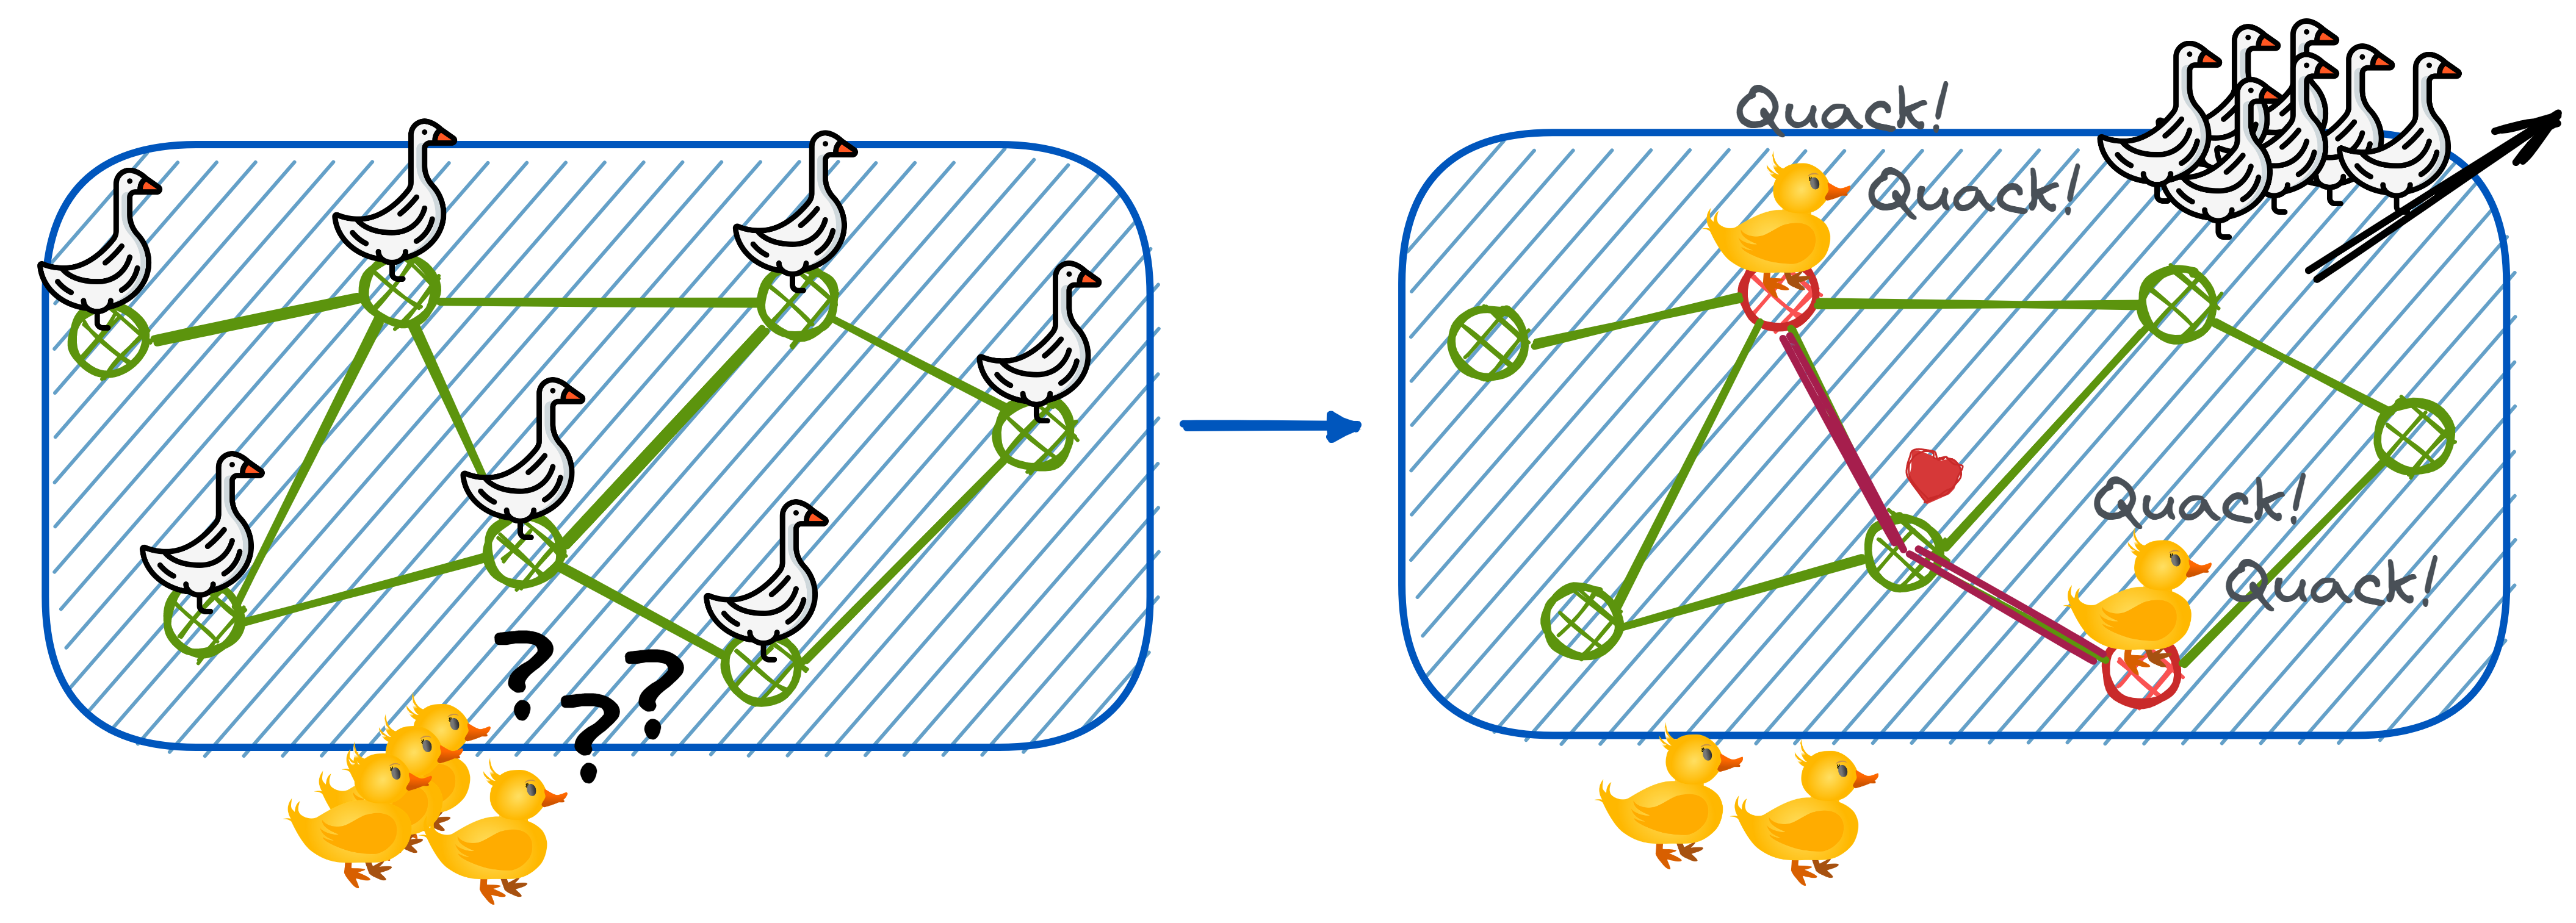
\includegraphics[width=0.9\columnwidth]{excalidraw/lake.png}
    \caption[Introductions: Merganser Lake. Own Drawing. Embedded icons under public domain from {\href{https://creazilla.com/}{https://creazilla.com/}}]{\textit{Left: All water lilies are occupied by members of the \textit{geesiosi} clan! The handwritten arrows have been your first solution proposal which was refused by the \textit{Supreme Duck Decision Board}.
    Right: Your second and final solution: Two ducks are enough to make all \textit{geesiosi}s flee. Furthermore, they are only two water lilies apart (red line) and therefore have someone to quack together with!}}
    \label{fig:duck-lake}
\end{figure}

Back in your library, you learn from some ancient scrolls that this problem has already been formalized by a professor called Henning \cite{Henning2019} as the \sdom problem, which is a variant of the intensively studied \dom problem. 
You read that both problems are \NPc~\cite{Garey1979,Henning2019}, and they are probably tough to solve in the general case efficiently, but there might still be hope if additional information is known. 
You look back into the map (\cref{fig:duck-lake}) and observe that none of the `quacking'-relations do cross with each other, and you are getting curious if it can be used for something\ldots

\section{Content of the Thesis}

Emerged during the last two decades, \textit{parameterized complexity} is a modern branch of computer science that showed many practical implications. 
This thesis systematically analyzes the \sdom problem through the lens of \textit{parameterized complexity}. 

\begin{itemize}
    \item \Cref{ch:prelim} will give the necessary definitions in the fields of \textit{graph theory} and \textit{parameterized complexity}.
    \item In \cref{ch:semitotal-domination}, we will discuss the \sdom problem and its relation to \dom and \tdom in more detail. 
    As they are closely related, we will gather the complexity status for various graph classes and compare them with each other in \cref{ch:complexity-status}. 
    We will then show $\WTWO$-intractability for general, bipartite, split (and chordal) graphs.
    \item \Cref{ch:linkern} is the mainstay of this thesis. 
    We are going to construct a linear kernel for \psdom following an approach first suggested by Alber, Fellows and Niedermeier \cite{Alber2004}. 
    \item In \cref{ch:closing}, we will give further ideas on how to improve the kernel and an outlook about interesting open problems for \sdom in general.
\end{itemize}


\paragraph{Our contributions}

While many authors have already stated positive results - for example, there exist polynomial-time algorithms for \emph{AT-free}, \emph{block} and \emph{interval} graphs as well as for \emph{graphs of bounded mim-width} and \emph{graphs of bounded clique-width} \cite{Kloks2021, Galby2020,Courcelle1990,Henning2022,Henning2019} - \NP-completeness was shown for various graph classes like general graphs, \emph{split}, \emph{planar}, \emph{chordal bipartite} and \emph{circle} graphs \cite{Henning2019, Kloks2021}.


We will further investigate these \NPc cases by applying the framework of \textit{parameterized complexity}. 
We could show $\WTWOhs$-intractability for \textit{general}, \textit{bipartite}, \textit{chordal}, \textit{split}, and \textit{perfect graphs} using parameterized reductions from \dom when parameterized by solution size.

In a groundbreaking paper, Alber, Fellows, and Niedermeier \cite{Alber2004} first gave a linear kernel for \pdom. 
They discovered that a planar graph can be decomposed into a linear number of smaller regions. 
This motivated the introduction of local reduction rules that shrink the number of vertices in such a region to a constant size. 
Following up on this result, a plethora of other explicit linear kernels for domination problems on planar graphs were found \cite{Guo2007, Garnero2017, Luo2013, Alber2006} and it made us believe we can also transfer them to \psdom.
Our hunch turned out to be true, and by adjusting the reduction rules given by Garnero and Sau \cite{Garnero2018}\footnote{We will rely on two different versions of this paper throughout the thesis. The \textit{arXiv} versions are explicitly marked.} for \ptdom, we were able to give an explicit kernel for \psdom of size $\kernelsize k$. 
More precisely, we are going to prove the following theorem:

\begin{restatable}[]{theorem}{centraltheo}\label{thm:central}
    The \sdom problem parameterized by solution size admits a linear kernel on planar graphs. There exists a polynomial-time algorithm that, given a planar graph $(G, k)$, either correctly reports that $(G, k)$ is a NO-instance or returns an equivalent instance $(G', k)$ such that $\abs{V(G')} \leq \kernelsize \cdot k$.
\end{restatable}